% Figure 5.8: Skill-Course NCF Architecture
% Compile with: pdflatex fig_5_8_skill_course_ncf.tex

\documentclass[border=10pt]{standalone}
\usepackage{tikz}
\usetikzlibrary{shapes.geometric, arrows.meta, positioning}
\usepackage{xcolor}

% Professional academic color palette
\definecolor{inputgray}{RGB}{220, 220, 220}
\definecolor{embedblue}{RGB}{176, 196, 222}    % Light steel blue
\definecolor{denseorange}{RGB}{222, 184, 135}  % Burlywood
\definecolor{outputpurple}{RGB}{186, 175, 201} % Lavender gray
\definecolor{accentteal}{RGB}{119, 176, 166}   % Muted teal
\definecolor{layer2}{RGB}{100, 149, 237}       % Cornflower blue
\definecolor{textdark}{RGB}{33, 33, 33}

\begin{document}
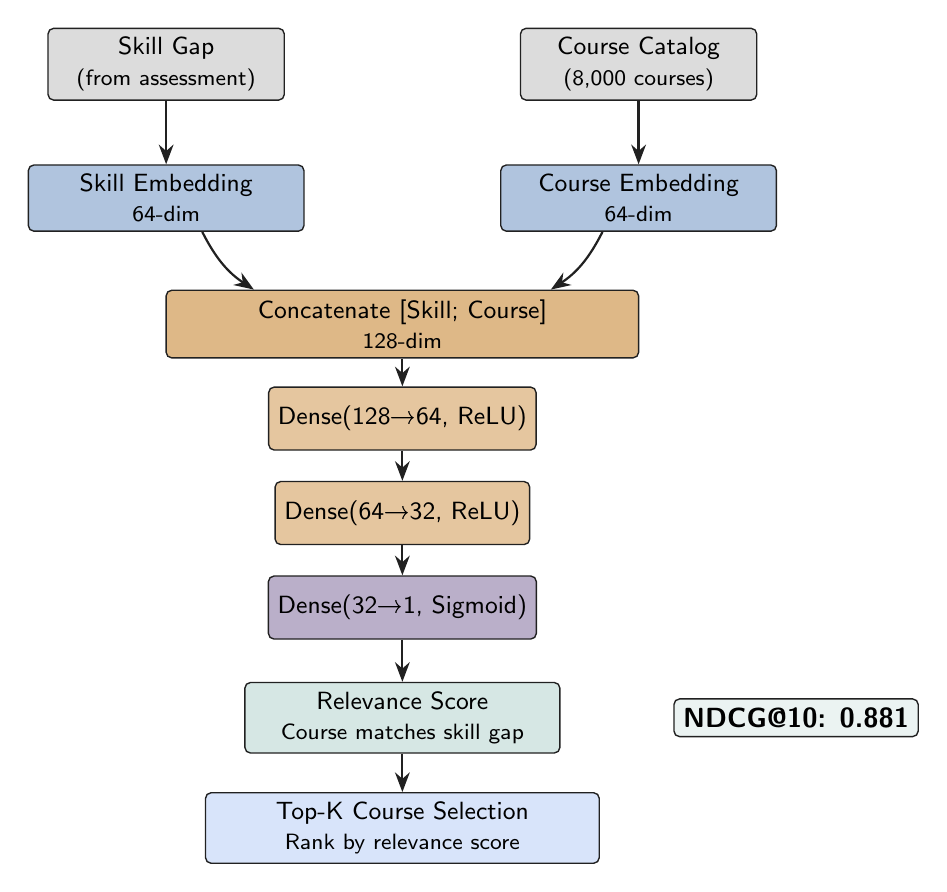
\begin{tikzpicture}[
    node distance=1cm,
    layer/.style={rectangle, draw=textdark, rounded corners=2pt, minimum width=3cm, minimum height=0.8cm, align=center, font=\small\sffamily, line width=0.5pt},
    arrow/.style={-{Stealth[length=2.5mm]}, thick, color=textdark},
]

% Skill input
\node[layer, fill=inputgray] (skill) at (-3, 5.5) {Skill Gap\\{\footnotesize\sffamily (from assessment)}};

% Course input  
\node[layer, fill=inputgray] (course) at (3, 5.5) {Course Catalog\\{\footnotesize\sffamily (8,000 courses)}};

% Embeddings
\node[layer, fill=embedblue, minimum width=3.5cm] (skillemb) at (-3, 3.8) {Skill Embedding\\{\footnotesize\sffamily 64-dim}};
\node[layer, fill=embedblue, minimum width=3.5cm] (courseemb) at (3, 3.8) {Course Embedding\\{\footnotesize\sffamily 64-dim}};

\draw[arrow] (skill) -- (skillemb);
\draw[arrow] (course) -- (courseemb);

% NCF layers
\node[layer, fill=denseorange, minimum width=6cm] (concat) at (0, 2.2) {Concatenate [Skill; Course]\\{\footnotesize\sffamily 128-dim}};

\node[layer, fill=denseorange!80] (mlp1) at (0, 1) {Dense(128→64, ReLU)};
\node[layer, fill=denseorange!80] (mlp2) at (0, -0.2) {Dense(64→32, ReLU)};
\node[layer, fill=outputpurple] (out) at (0, -1.4) {Dense(32→1, Sigmoid)};

\node[layer, fill=accentteal!30, minimum width=4cm] (score) at (0, -2.8) {Relevance Score\\{\footnotesize\sffamily Course matches skill gap}};

\draw[arrow] (skillemb) to[bend right=15] (concat);
\draw[arrow] (courseemb) to[bend left=15] (concat);
\draw[arrow] (concat) -- (mlp1);
\draw[arrow] (mlp1) -- (mlp2);
\draw[arrow] (mlp2) -- (out);
\draw[arrow] (out) -- (score);

% Top-K selection
\node[layer, fill=layer2!25, minimum width=5cm] (topk) at (0, -4.2) {Top-K Course Selection\\{\footnotesize\sffamily Rank by relevance score}};
\draw[arrow] (score) -- (topk);

% Best NDCG annotation
\node[rectangle, draw=textdark, fill=accentteal!15, rounded corners=2pt, font=\sffamily, line width=0.5pt] at (5, -2.8) {\textbf{NDCG@10: 0.881}};

\end{tikzpicture}
\end{document}
